\chapter{Introducción}

\drop{E}{n} la actualidad, cada vez es más frecuente escuchar hablar del talento humano de las empresas. Éste es el mejor recurso de estas,
 los empleados son los que mejor conocen su trabajo y pueden tener ideas de como mejorar diversos aspectos de la empresa. 
 
 Los clásicos buzones de sugerencias pueden servir a las empresas para conocer las mayores molestias de
  algunos de sus empleados. Estos rápidamente pueden convertirse en buzones de quejas, o los empleados pueden
   sentir que no se toman en cuenta sus opiniones si estas  sugerencias o quejas no obtienen una respuesta.
 
 Un \acf{SMI} puede ayudar a las empresas a fomentar la innovación desde cualquiera de los miembros de 
 estas. Además, «contar con información sobre la opinión de los empleados permite evitar errores en la toma
  de decisiones, y ayuda a dirigir los esfuerzos de mejora allí donde la organización detecta problemas»
   \cite{talento}. Los principales beneficios de estos sistemas son:
 
 \begin{itemize}
 	\item Aumento del compromiso de los empleados. 
 	\item Promueve la transparencia dentro de la empresa. Cada una de los miembros de la organización
 	puede aportar sus ideas sin necesidad de pasar por 	su "jefe". Todos los usuarios tienen la misma
 	 importancia y visibilidad.
 	\item Permite a los empleados dar su opinión. Todos los empleados en la compañía pueden proponer sus  ̈cambios y mejoras en Nextinit.
 	\item Detecta el talento. La organización detecta cuáles de sus miembros tienen
 	mayor talento para llevar a cabo esas iniciativa de mejora planteadas en la herramienta.
 	\item Retiene el talento. Nextinit ayuda a retener el talento, pues los miembros de la organización
 	 ven como sus propuestas son tomadas en consideración y como aquellas que han conseguido el apoyo de
 	  sus compañeros se implantan.
 	\item Mejora el clima laboral. Nextinit hace que los miembros de la organización colaboren entre sí 
 	para sacar adelante las ideas, por tanto mejora el clima laboral.
 	\item Alinea todos los empleados con los objetivos estratégicos de la compañía. La empresa puede definir cuales son sus prioridades estratégicas en Nextinit, de tal manera que cada una de las ideas 
 	cumplirá un porcentaje de cada una de las prioridades estratégicas establecidas (ver Figura~\ref{fig:prioridades}).
 	\item Genera ideas apoyadas por los empleados para mejorar la empresa en ámbitos muy diversos.
 \end{itemize}

\begin{figure}[!h]
	\begin{center}
		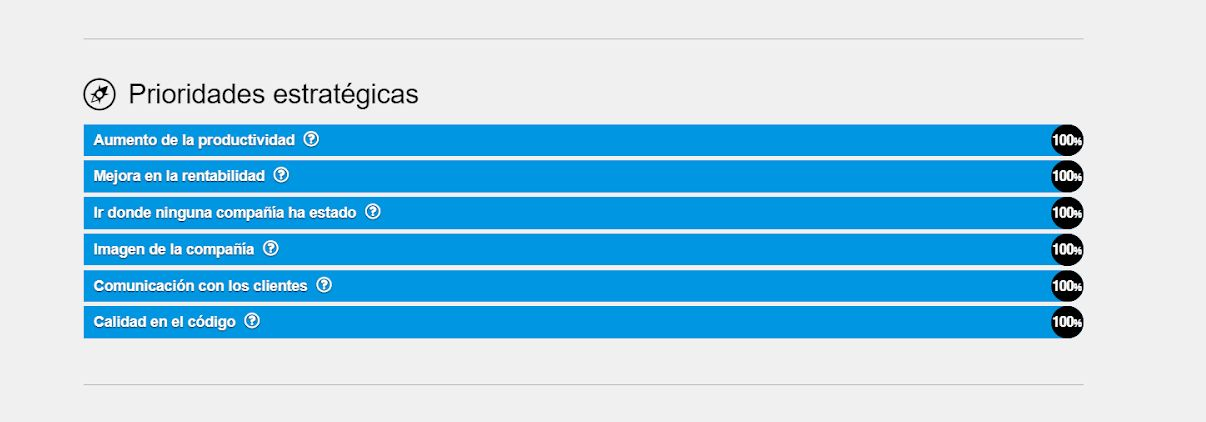
\includegraphics[width=0.8\textwidth]{./img/introduccion/prioridades.png}
		\caption{Ejemplo de prioridades estratégicas en Nextinit}
		\label{fig:prioridades}
	\end{center}
\end{figure}
 
 
 \section{Nextinit}
 
 Nextinit es un \acs{SMI}, una herramienta que permite que cualquier miembro de una organización pueda
 proponer ideas para  mejorarla y resolver desafíos lanzados por esta. Las ideas se crean dentro de la 
 plataforma de forma similar a una startup que busca dinero. Los usuarios no solo pueden  proponer ideas, sino 
 invertir dinero virtual para que las ideas propuestas en la plataforma aumenten el capital invertido   y 
 puedan salir adelante.
 
 La idea de esta plataforma es usar la inteligencia colectiva para mejorar las organizaciones. Como el dinero 
 virtual de cada usuario es limitado, estos solo invertirán,  en las mejores ideas, por lo que si mucha gente 
 invierte en una idea, será porque dicha idea es buena. Y si esa idea se lleva a cabo se recupera el dinero 
 invertido  mas unos intereses.
 
 Las organizaciones pueden publicar desafíos, que consiste en pedir ideas a los usuarios para un 
 objetivo o tema concreto. Las ideas dentro de los desafíos que elija la organización puede dar 
 recompensas como un \acs{ROI} más alto que el habitual sino también premios especiales elegidos
 por la organización.
  
  Además, dispone de un sistema de gamificación, en que se van obteniendo medalas conforme van
  consiguiendo unas metas establecidas, como publicar o que un usuario lance su primera idea. También
   dispone de sistemas de \textit{rankings} que fomentan la competencia entre usuarios.
   
 \subsection{Flujo de ideas}
 
 La publicación y selección de ideas sigue el siguiente flujo (ver Figura~\ref{fig:flujo}):
 
 \begin{figure}[!h]
 \begin{center}
 
\includegraphics[width=0.8\textwidth]{./img/introduccion/flujo.png}
 \caption{Fases de una idea}
 \label{fig:flujo}
 \end{center}
 \end{figure}
 
 \begin{enumerate}
 	\item Un usuario publica una idea y automáticamente esta empieza a buscar financiación. El sistema calcula la cantidad de dinero que deberá conseguir para destacar de entre las demás.
 	\item Si se consigue la cantidad de dinero necesaria (o si lo considera la organización), el equipo de
 	 innovación de la organización decide si desarrolla un proyecto piloto o no.
 	 \item Si supera la fase piloto, la idea será implementada por la organización.
 	 \item Cada vez que la idea cambia entre las fases, los inversores reciben un \afc{ROI}, que permite
 	 que puedan seguir invirtiendo en otras ideas.
 \end{enumerate}
 
  
 
\section{Estructura del documento}

El presente documento se compone con la siguiente estructura:

\begin{definitionlist}
\item[Capítulo \ref{chap:objetivos}: \nameref{chap:objetivos}] Se expone el objetivo principal y sus subjetivos.
 \item[Capítulo \ref{chap:antecedentes}: \nameref{chap:antecedentes}] Se describen los sistemas tomados como referencia utilizados para 
 el desarrollo de este \acs{TFG}.
  \item [Capítulo \ref{chap:metodo}: \nameref{chap:metodo}] Se describe y justifica la metodología utilizada para el desarrollo de este \acs{TFG}.
  \item[Capítulo \ref{chap:resultados}: \nameref{chap:resultados}] Se muestran los resultado obtenidos al aplicar la metodología elegida.
  \item[Capítulo \ref{chap:conclusiones}: \nameref{chap:conclusiones}] Se exponen las conclusiones llegadas al finalizar el desarrollo.
\end{definitionlist}

% Local Variables:
%  coding: utf-8
%  mode: latex
%  mode: flyspell
%  ispell-local-dictionary: "castellano8"
% End